\chapter{Stoss}
\label{v:1}

In diesem Versuch werden die Grundlagen des inelastischen Sto{\ss}es am Beispiel eines Fadenpendels studiert. Das Fadenpendel ist auch heute noch eines der genauesten Instrumente zur Bestimmung der Erdbeschleunigung.

%\noindent
%{\bf Kenntnisse}: ???

%------------------------------------------------
\section{Stichworte}
%------------------------------------------------
Hubarbeit; Fadenpendel; pot. und kinet. Energie; Energiesatz; Impulssatz; elast. und inelast. Sto{\ss}.
%
%------------------------------------------------
\section{Literatur}
%------------------------------------------------
Gehrtsen, Kapitel 1.4.2/3, 1.5.2 bis 1.5.9; Demtr"oder, Kapitel 2.1, 2.2, 4.2
%
%------------------------------------------------
\section{Anwendungsbeispiele}
%------------------------------------------------
%
Beim inelastischen Stoß zweier Körper wird ein Teil der zur Verfügung stehenden Energie (die Summe der kinetischen Energien der beiden Körper vor dem Stoß) in Innere Energie der Körper umgewandelt. Das kann durch Erwärmung oder Verformung der Körper geschehen.\\
Beispiele für solche inelastischen Stoßvorgänge sind die Formung chemischer Verbindungen aus mehreren Atomen oder Molekülen in Gasen oder Flüssigkeiten, das Auffalten von Gebirgen beim Zusammensto{\ss} tektonischer Platten oder auf kleineren Skalen der Blechschaden beim Zusammensto{\ss} von Fahrzeugen. Ein weiteres Beispiel ist die mit der Zeit abnehmende Sprunghöhe eines elastischen Balls, der vom Boden abprallt.\\
Wir betrachten inelastische Stöße am Beispiel des Fadenpendels, anhand dessen sehr viele Eigenschaften von schwingenden Systemen verdeutlicht werden können. Einer der interessantesten Aspekte ist zum Beispiel die Unabhängigkeit der Schwingungsdauer des Pendels von der Masse des schwingenden Körpers, s. Pendeluhren oder Spiderman.\\

Auch wenn die theoretische Einleitung etwas länger ist als bei anderen Versuchen, ist es doch sinnvoll sich mit den Grundlagen der Bewegung von Massepunkten (geworfene Bälle, Sie, Autos, etc.) zu beschäftigen. Diese Gesetzmäßigkeiten betreffen nicht nur jeden einzelnen von uns im Alltag, sondern bilden die Grundlagen für Effekte in allen Naturwissenschaften.
%
%------------------------------------------------
\section{Theoretischer Hintergrund}
%------------------------------------------------

\subsection{Die Kinematik von Massepunkten}

Die Kinematik ist die Lehre der Bewegung von Punkten und K"orpern im Raum, beschrieben durch die Gr"o{\ss}en Position, Geschwindigkeit und Beschleunigung.\\
Den Gr"o{\ss}en Position, Geschwindigkeit und Beschleunigung bei einer geradlinigen Bewegung entsprechen bei einer Drehbewegung die Gr"o{\ss}en Winkel, Winkelgeschwindigkeit und Winkelbeschleunigung.

Die Position eines Punktes wird durch drei Koordinaten im dreidimensionalen Raum festgelegt. Bei einem starren K"orper (der sich nicht verformt) gen"ugen drei weitere Freiheitsgrade f"ur die Rotation (Drehungen im dreidimensionalen Raum), um die Lage des gesamten K"orpers zu beschreiben. Die drei Koordinaten eines Ortes stellt man durch die drei Komponenten eine Vektors dar:\\
Die Koordinaten (x,y,z) entsprechen dem Ort $\vec{x} = (x,y,z)$. Mit der Schreibweise $\vec{x}(t)$ bezeichnet man den Ort des K"orpers zu einer bestimmten Zeit $t$. Tr"agt man nun diese Funktion gegen die Zeit $t$ auf, so bekommt man die sogenannte \textit{Bahnkurve} des K"orpers. Geschwindigkeit und Beschleunigung sind definiert als Ableitungen der Ortskurve nach der Zeit:
\begin{align}
\vec{v}(t) & = \dot{\vec{x}}(t) = \frac{d\vec{x}(t)}{dt} = \left(\frac{dx}{dt}, \frac{dy}{dt}, \frac{dz}{dt}\right) \\
\vec{a}(t) & = \ddot{\vec{x}}(t) = \frac{d^2\vec{x}(t)}{dt^2} = \left(\frac{d^2x}{dt^2} , \frac{d^2y}{dt^2}, \frac{d^2z}{dt^2}\right)
\end{align}

\subsection{Grundlagen von Schwingungen}

Verschiebt man einen elastisch gebundenen Körper aus seiner Ruhelage (z. Bsp. an einer Feder herabhängende Masse nach oben oder unten, die Masse eines Fadenpendels zur Seite), dann bewegt er sich nach dem Loslassen beschleunigt auf seine Ruhelage zu und läuft aufgrund seiner Trägheit über diese hinaus. Nach dem Durchgang durch die Ruhelage wirkt die rücktreibende Kraft verzögernd, da sie jetzt der Bewegungsrichtung entgegengesetzt ist und der Körper kommt schließlich zur Ruhe (Umkehrpunkt). Jetzt wiederholt sich der Bewegungsablauf in umgekehrter Richtung, bis der Ausgangspunkt erreicht ist (wenn Reibung vernachl"assigt wird). \\
Diesen periodisch wiederkehrenden Vorgang nennt man Schwingung, die Zeit $T$, die verstreicht bis sich ein Bewegungszustand (bestimmt durch Ort, Betrag und Richtung der Geschwindigkeit) wieder einstellt, hei{\ss}t Schwingungsdauer. Die Frequenz einer Schwingung ist definiert durch
\begin{equation}
f = 1/T \; ,
\end{equation}
ihre Kreisfrequenz $\omega$, auch Winkelfrequenz genannt, durch
\begin{equation}
\omega = 2\pi f = 2\pi /T\; .
\end{equation}
%
\begin{hint}
Winkel werden entweder in Einheiten von Grad oder von Radiant angegeben. In der alltäglich gebräuchlicheren Einheit entspricht eine volle Umdrehung um eine Achse 360° (Grad).\\
Das Rechnen mit Winkeln wird allerdings sehr viel einfacher, wenn man diese in der dimensionslose Einheit von Radiant angibt. In dieser Einheit entspricht eine volle Umdrehung $2\pi$~rad. Die Umrechnung von Winkeln in Grad nach Radiant ist gegeben durch
\begin{equation}
	\varphi \mathrm{\left[rad\right]} = \varphi \mathrm{\left[grad\right]}*\frac{2\pi}{360^{\circ}} \; .
\end{equation}
Die oben eingeführte Frequenz $f$ gibt an, wie oft pro Sekunde ein kompletter Schwingungsvorgang durchlaufen wird. Beim Fadenpendel zum Beispiel, wie oft sich das Pendel vom linken Umkehrpunkt zum rechten und zurück bewegt. Die Kreisfrequenz $\omega$ hingegen gibt an, welcher Anteil des gesamten Schwingungsvorgangs pro Sekunde zurückgelegt wird.\\Die Einheit der Frequenz ist das \textit{Hertz}, mit $1 \mathrm{H} = 1/\mathrm{s}$, während die Einheit der Kreisfrequenz \textit{Radiant pro Sekunde} ist.
\end{hint}
%
Man unterscheidet zwischen harmonischen und anharmonischen Schwingungen, je nachdem, ob die r"ucktreibende Kraft linear oder nichtlinear von der Auslenkung abh"angt. Eine Schwingung, deren Amplitude durch Energieverlust (zum Beispiel aufgrund von Reibung) monoton abnimmt, hei{\ss}t ged"ampfte Schwingung. Sie ist kein periodischer Vorgang, da der Ausgangspunkt der Bewegung nicht wieder erreicht wird. Erzwungene Schwingungen sind solche, bei denen durch Energiezufuhr von au{\ss}en ein System zum schwingen angeregt bzw. trotz D"ampfung in einem station"aren Schwingungszustand gehalten wird.

Man kann auch die Energie des Pendels im Verlauf einer Pendelschwingung betrachten. Wird das Pendel ausgelenkt, so wird der K"orper dadurch ein wenig angehoben. Da dabei Arbeit gegen die Schwerkraft verrichtet wird, hat der K"orper im angehobenen Zustand, also wenn das Pendel ausgelenkt ist, eine gr"o{\ss}ere potenzielle Energie, als wenn es nicht ausgelenkt ist. Die zus"atzliche potenzielle Energie betr"agt $E_{pot} = m\cdot g\cdot h = m\cdot g\cdot l(1-\cos\varphi)$. In diesem Moment bewegt sich der K"orper nicht, so dass er keine kinetische Energie besitzt.\\
Wird der K"orper nun losgelassen wird er in einer beschleunigten Bewegung auf die Ruhelage zu fallen. In dem Moment, wo der K"orper die Ruhelage passiert, seine H"ohe "uber dem Erdboden also wieder dieselbe ist wie vor der Auslenkung, hat er kein zus"atzliche potenzielle Energie mehr. Stattdessen bewegt er sich hier mit seiner maximalen Geschwindigkeit $v_{max}$. Demnach hat er die kinetische Energie $E_{kin} = \frac{1}{2}m\cdot v_{max}^2$. \\
Die gesamte zus"atzliche potenzielle Energie, die der K"orper in der ausgelenkten Position hatte, ist in diesem Moment komplett in kinetische Energie verwandelt.

\subsection{Das Fadenpendel}

Das Fadenpendel besteht aus einer Kugel der Masse $m$, die an einem Faden der L"ange $L$ (gemessen zwischen Aufh"angepunkt und Mittelpunkt der Kugel) h"angt. Wenn die Masse des Fadens vernachl"assigbar ist gegen $m$ und der Durchmesser der Kugel sehr klein gegen"uber der Fadenl"ange L ist, hei{\ss}t die Anordnung \emph{mathematisches Pendel}, weil $m$ als Punktmasse behandelt werden kann.\\
Die Bewegung des Pendels unter dem Einfluss der Schwerkraft kann man sich wie folgt klarmachen:\\ 
An der aus der Ruhelage um den Winkel $\varphi$ herausgedrehten Kugel greift die Schwerkraft $\vec{F}_s = m\vec{g}$ an. Man zerlegt die Schwerkraft in zwei Komponenten
\begin{itemize}
 \item eine radiale Komponente $F_r$, die im gespannten Faden eine gleich gro{\ss}, entgegengerichtete Kraft hervorruft und deshalb nichts zur Beschleunigung beitr"agt,
 \item eine tangentiale Komponente $F_t = -m\cdot g\cdot\sin\varphi$, die eine Tangentialbeschleunigung \\
 $a_t = -g\cdot\sin\varphi$ bewirkt. Dies ist die r"ucktreibende Kraft.
\end{itemize}
%
In ebenen Polarkoordinaten lautet die Bewegungsgleichung des Pendels:
\begin{equation}
m\cdot g\cdot\sin\varphi = -m\cdot L\cdot \ddot{\varphi}
\end{equation}
%
Entwickelt man $\sin\varphi$ in die Taylorreihe
\begin{equation*}
\sin\varphi = \varphi - \frac{\varphi^3}{3!}+ \frac{\varphi^5}{5!} - \frac{\varphi^7}{7!}+ ...
\end{equation*}
so kann man f"ur gen"ugend kleine Werte von $\varphi$ die h"oheren Glieder vernachl"assigen. Damit wird die Bewegungsgleichung zu:
\begin{equation}
\ddot{\varphi} = - \frac{g}{L}\cdot\varphi \; .
\end{equation}
Die L"osung dieser Differentialgleichung ist die Funktion
\begin{equation}
\varphi (t) = \varphi_0\cdot\sin\omega t \;.
\end{equation}
%
$\varphi_0$ ist dabei die ursprüngliche Winkelauslenkung. Die Kreisfrequenz der Schwingung ist dabei $\omega = \sqrt{g/L}$, die Schwingungsdauer oder \emph{Periode} der Schwingung wird $T = \frac{2\pi}{\omega} = 2\pi\cdot\sqrt{L/g}$. Wie man sieht, ist die Periode also nicht von der Auslenkung oder der Masse abhängig, sondern nur von der Fadenlänge und der Erdbeschleunigung.

Diese Tatsache ist die Grundlage der Funktion von Pendeluhren, welche im 18. Jahrhundert besonders in der Seefahrt eine große Rolle spielten, weil sie zum die objektive Zeitmessung auf hoher See, und damit die genaue Bestimmung des Längengrades erlaubten. Das englische Parlament hatte im Jahr 1714 ein Preisgeld von 20.000 Pfund für die Lösung des sogenannten Längenproblems (die genaue Bestimmung des aktuellen Längengrades) ausgelobt, welches sich der Tischler, Erfinder und autodidaktische Uhrmacher John Harrison erst im Jahre 1765 nach langem Streit teilweise ausgezahlt bekam. Die von ihm erfundene Uhr erreichte eine damals enorm hohe Genauigkeit (etwa 1 Sekunde Abweichung pro Monat).
%
\begin{figure}[hb]
	\centering
		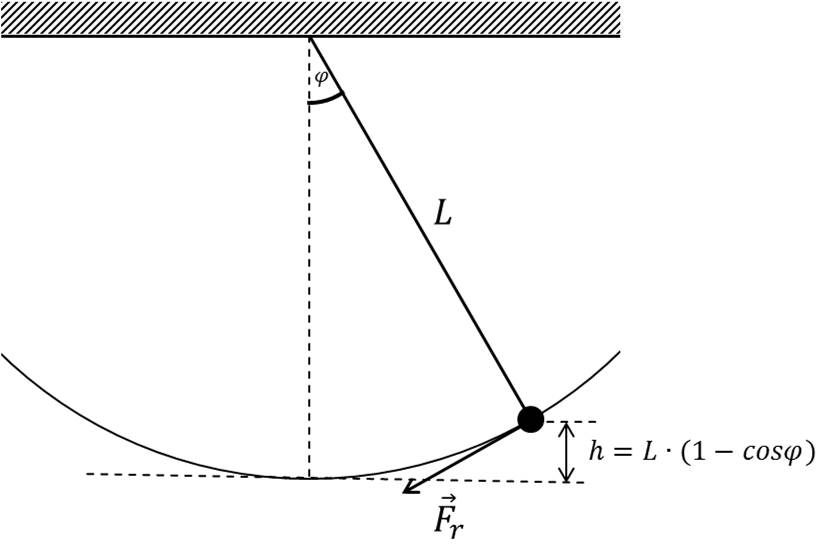
\includegraphics[height=6cm]{Abbildungen/Fadenpendel.jpg}
	\caption{Fadenpendel}
	\label{fig:Fadenpendel}
\end{figure}

\subsection{St"o{\ss}e zwischen zwei K"orpern}

Ein Stoß ist eine sehr kurzzeitige Wechselwirkung zwischen zwei Körpern. Vor und nach dem Stoß bewegen sich beide, ohne einander zu beeinflussen. Obwohl die Gesamtenergie der beiden Sto{\ss}partner immer erhalten ist, kann h"aufig ein Teil der kinetischen Energie beim Sto{\ss} in andere Energieformen, z.B. in potenzielle Energie oder in W"armeenergie umgewandelt werden. Der Gesamtimpuls der beiden bleibt jedoch beim Sto{\ss} immer erhalten. Die Grundgleichungen f"ur Sto{\ss}prozesse zwischen zwei K"orpern lassen sich also schreiben als:
\begin{align}
\vec{p}_1^{'} + \vec{p}_2^{'} &= \vec{p}_1 + \vec{p}_2 &\mathrm{Impulssatz}\\
\frac{p_1^{'2}}{2m_1} + \frac{p_2^{'2}}{2m_2} &= \frac{p_1^{2}}{2m_1} + \frac{p_2^{2}}{2m_2} &\mathrm{Energiesatz}
\end{align} 
%
Hierbei bezeichnen gestrichene Gr"o{\ss}en (z.B. $\vec{p}_1^{'}$) auf die Gr"o{\ss} nach dem Stoss. Beachten Sie, dass wir bei dieser klassischen Form des Energiesatzes die innere Energie nicht ber"ucksichtigt haben.\\
%
\begin{hint}
	Es sei an die Definitionen von kinetischer Energie und Impuls erinnert:
	\begin{align}
		\vec{p} &= m\cdot\vec{v}\\
		E_{kin} &= \frac{1}{2}mv^2 
	\end{align}
\end{hint}
%
Anhand der Energien der beiden Stoßpartner unterscheidet man drei Situationen:
\begin{enumerate}
	\item \textbf{Elastischer Stoß:}\\
		Die kinetische Energie beider Stoßpartner ist nach dem Stoß genauso groß wie davor. Beispiele hierfür sind die meisten Zusammenstöße von Molekülen, roten Blutkörperchen oder ähnlichem, die Rammbockkämpfe vieler Tierarten, oder die Brown'sche Bewegung.
	%
	\item \textbf{Inelastischer Stoß:}\\
		Ein Teil der kinetischen Energie der Stoßpartner wird dauerhaft in eine andere Energieform überführt, wie zum Beispiel Erwärmung oder Verformung. Beispiele hierfür wären die Überdehnung einer Sehne oder der Bruch eines Knochens, chemische Reaktionen, oder das Hämmern eines Spechts.
	%
	\item \textbf{Vollständig inelastischer Stoß:}\\
		Hierbei verbinden sich die Stoßpartner miteinander, sodass sie sich im Folgenden mit einer gemeinsamen Geschwindigkeit weiterbewegen. Beispiele sind die Untereinheiten von Ribosomen, die sich miteinander verbinden, sowie die beiden Metallkugeln im Versuch, welche nach dem Stoß durch die Knetmasse verbunden sind.
	%
\end{enumerate}
%------------------------------------------------
\section{Fragen zur Vorbereitung}
%------------------------------------------------

\begin{enumerate} 
% \item Was soll heute im Praktikum gemessen werden? Warum?
 %
 \item Welche mechanischen Gr"o{\ss}en ben"otigt man, um die Bewegung eines K"orpers zu beschreiben?
 %
 \item Wie stehen Ort, Geschwindigkeit und Beschleunigung eines K"orpers im Zusammenhang?
 %
 \item Wie lauten die Formeln f"ur die kinetische und die potentielle Energie?
 %
 \item Warum gilt beim inelastischen Stoss nur der Impuls-, nicht aber der Energiesatz?
 %
 \item Wie kommt die Formel $L=\frac{T^2\,g}{4\,\pi^2}$ zustande?
 %
 \item Wie lautet das Gravitationsgesetz?
\end{enumerate} 

%------------------------------------------------
\section{Durchführung} 
%------------------------------------------------

Die Masse der großen Kugel beträgt $M = 2,10$\,kg, die der kleinen Kugel beträgt $m=0,11$\,kg.

\begin{enumerate}
%
\item Bestimmen Sie die Schwingungsdauer T des Pendels, indem Sie fünfmal die Zeit für 10 ganze Schwingungen messen. Die horizontale Auslenkung des Pendels soll dabei nicht größer sein als etwa 40~cm. Warum? Wie groß ist der Fehler Ihrer Messung? \label{Mess:Schwingungsdauer}
%
\item An der großen Kugel wird die Knetmasse so befestigt, dass die ausgelenkte kleine Kugel zentral auf die Knetmasse stößt und dann beide Kugeln samt Knetmasse nach dem unelastischen Stoß gemeinsam ausschwingen. Die Auftreffgeschwindigkeit der kleinen Kugel wird variiert, indem man die Fallhöhe $h$ verändert ($h$ = 3, 4, 5, 6~cm). In Abhängigkeit von der Fallhöhe $h$ der kleinen Kugel ist dann der maximale Ausschlag x$_0$ der beiden Kugeln samt Knetmasse nach dem zentralen Stoß zu messen. Schätzen Sie den Fehler Ihrer Messung ab.
\label{Mess:inelast_Stoss}
%
\item Messen Sie die Masse der Knetmasse $m_k$. Wie groß ist die Unsicherheit?
%
\item Notieren Sie die Länge des Fadens, an dem der Pendelkörper aufgehängt ist. Diese können Sie als genau bekannt annehmen.
%
\end{enumerate}

%------------------------------------------------
\section{Auswertung} 
%------------------------------------------------

\begin{enumerate}
%
\item Berechnen Sie aus der Messung \ref{Mess:Schwingungsdauer} die Erdbeschleunigung $g$. Wie gro{\ss} ist der Fehler Ihrer berechneten Größe? Siehe hierzu Kapitel \ref{chap:Fehlerfortpflanzung}. Vergleichen Sie diese mit dem Literaturwert und diskutieren Sie Gr"unde m"oglicher Abweichungen.
%
\item In Abh"angigkeit von der Fallh"ohe $h$ berechne man die Geschwindigkeit $v_m$ der kleinen Kugel beim Auftreffen auf die gro{\ss}e Kugel.
%
\item Nach dem inelastischen Stoss bewegen sich alle Massen (einschlie{\ss}lich Knete!) mit einer gemeinsamen Geschwindigkeit $v_{th}$. Berechnen Sie diese Geschwindigkeit mithilfe des Impulssatzes 
\begin{equation}
\label{Gl:Impulssatz}
(M + m + m_k)\cdot v_{th} = m\cdot v_m\; .
\end{equation}
(Machen Sie sich klar, dass Gleichung \ref{Gl:Impulssatz} wirklich dem Impulssatz entspricht.)
%
\item Bestimmen Sie die Geschwindigkeit $v_{exp}$ der beiden Massen samt Knete aus dem maximalen Ausschlag $x_0$ in Messung \ref{Mess:inelast_Stoss} für alle Fallhöhen. Benutzen Sie die Beziehung:
\begin{equation}
v_{exp} = \frac{2\pi}{T}\cdot x_0\
\end{equation}
%
\item Vergleichen Sie die experimentellen und die theoretischen Geschwindigkeiten $v_{exp}$ und $v_{th}$ miteinander und geben Sie eine Erklärung für auftretende Differenzen ( = Fehlerbetrachtung).
%
\end{enumerate}